\section{Introduction}
\label{sec:introduction}

Every quantum learning experiment ends the same way: a circuit runs many
times, and each run returns one measured bitstring. Before anything can be
learned, this pile of shots must become training data. The step looks like
bookkeeping, and it is usually treated that way. Almost every pipeline averages
all shots of a time step into a single expectation-value estimate and moves on.
This paper argues that the step is not bookkeeping. It is a statistical decision
with measurable consequences, and treating it as a validated hyperparameter
improves finite-shot quantum learning at no additional quantum cost.

\begin{figure}[!t]
  \centering
  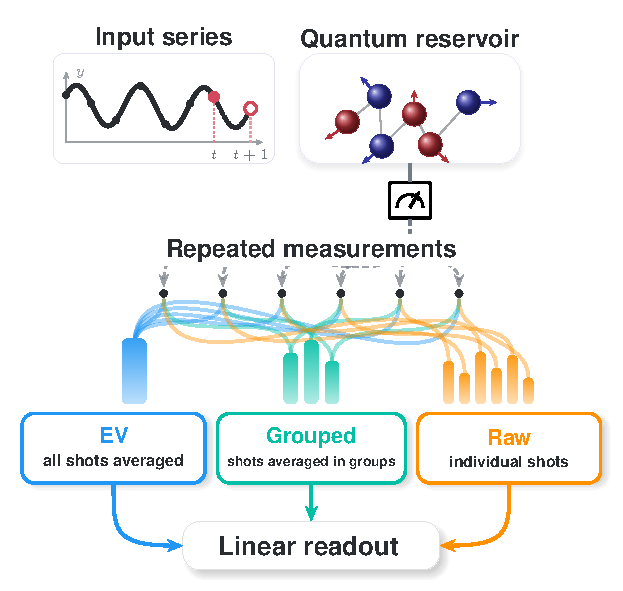
\includegraphics[width=\columnwidth]{fig1_shot_organization.pdf}
  \caption{Three ways to turn one shot record into training data. A fixed quantum
  reservoir is measured many times per step, and only the classical step changes:
  EV averages all shots, Raw keeps each shot, and Grouped averages disjoint groups.
  All feed the same linear readout.}
  \label{fig:organization}
\end{figure}

The averaging convention is well motivated, because expectation values are the
quantities predicted by theory and estimated in experiments. A learning
pipeline, however, does not consume observables. It consumes training examples,
and it cares about two things only: how many there are and how noisy each one is.
The moment a measurement record becomes training data, a physics convention
quietly turns into a statistical choice: spend all measurements on making one
example clean, or make several examples that are merely clean enough. No single
choice can suit every task, budget, and noise level.

Averaging everything is one end of a dial. It buys the cleanest possible feature
vector but pays with scarcity: thousands of circuit executions collapse into a
handful of training examples, and too few examples relative to the number of
features destabilizes regression~\cite{hsu2012random}. The opposite end, keeping
every shot as its own example, buys abundance but pays with noise, and noisy
features systematically shrink fitted coefficients~\cite{fuller1987measurement}.
Between these extremes lies an entire range of aggregations that quantum machine
learning usually leaves implicit.

\emph{Adaptive shot aggregation} makes this choice explicit. The $N$ shots of
each time step are partitioned into disjoint groups of size $k$ and averaged
within each group, so that a single parameter slides smoothly from raw shots
($k=1$) to full expectation-value averaging ($k=N$). The group size is a
validation-selected hyperparameter of the classical readout, chosen by
time-respecting validation jointly with the readout regularization. The
procedure operates purely on the classical record: it requires no new circuits,
no extra shots, and it can be applied retroactively to any archived record in
which individual outcomes were retained.

Quantum reservoir computing (QRC) is a clean place to study this
dial~\cite{fujii2017harnessing,nakajima2019boosting,mujal2021opportunities}. A
fixed quantum circuit transforms an input sequence into measured features, and
only a classical readout is trained. The circuit, the targets, and the
measurement record can therefore be held completely fixed while the aggregation
alone changes. Whatever happens to the forecast is attributable to the
aggregation, because nothing else moved. We compare three representations of
one record (Fig.~\ref{fig:organization}): the expectation-value representation
(EV), individual shots (Raw), and the grouped representation in between.

We find that the aggregation scale materially affects test error under fixed
execution budgets: at the balanced allocation, an intermediate scale lowers
mean test error relative to full averaging on all four evaluated forecasting
tasks, with paired confidence intervals above zero in every case. The best scale
depends on the record, so no single convention is appropriate. Matched controls
trace the gain to covariance regularization of the classical readout, supplied
automatically by the record's own shot fluctuations, and the effect transfers
to unmitigated experiments on real hardware. Our claims concern how to organize
a given measurement record, not quantum advantage.

In summary, this paper makes the following contributions:

\begin{itemize}
  \setlength{\itemsep}{1pt}
  \setlength{\parskip}{0pt}
  \setlength{\parsep}{0pt}
  \setlength{\topsep}{2pt}
  \item \textbf{A tunable aggregation procedure.} We make $k$ a
  validation-selected classical-readout hyperparameter spanning Raw to EV,
  chosen jointly with ridge strength and applicable retroactively at no added
  quantum cost (Sec.~\ref{sec:method}).

  \item \textbf{Evidence that the choice matters.} Under a fixed budget of
  10,000 executions, intermediate aggregation lowers mean error on all four
  tasks; a three-allocation sweep shows that gains are largest with many shots
  at few time steps
  (Secs.~\ref{sec:evaluation}-A and \ref{sec:evaluation}-B).

  \item \textbf{A mechanism.} An exact linear-readout identity equates grouped
  training with EV training plus a shot-covariance penalty; the matched
  Regularized EV control confirms this mechanism
  (Secs.~\ref{sec:method}-C and \ref{sec:evaluation}-C).

  \item \textbf{Transfer to hardware.} Unmitigated experiments with a separate
  ten-qubit reservoir on two processors show positive mean improvements on
  every task (Sec.~\ref{sec:evaluation}-D).
\end{itemize}
